%\documentclass[11pt,letterpaper]{article}
\documentclass[11pt,letterpaper]{llncs2e/llncs}
%\usepackage{floatrow}
%\DeclareFloatFont{normal}{\normalsize}
%\floatsetup{font=normal}
%\usepackage[normal]{caption}
%\usepackage{authblk}
\usepackage{indentfirst}
\usepackage[margin=1in]{geometry}
\usepackage{hyperref}
\usepackage{booktabs}
\usepackage[capitalise]{cleveref}
\usepackage{color}
\usepackage[dvipsnames]{xcolor}

\usepackage%[group-separator={\,}]
{siunitx}
\usepackage[noend]{algorithm2e}
\DontPrintSemicolon

\usepackage[sort,numbers]{natbib}
\renewcommand{\bibnumfmt}[1]{#1.}
%\bibliographystyle{IEEEtranN}
\usepackage{pgfplots}
\usepackage{gitinfo2}

%\usepackage[nolists,nomarkers]{endfloat}

\setcounter{secnumdepth}{6}

\title{FgClust, a fast and scalable algorithm for generating high-quality clusters of biological sequences}

\author{
	XiaoFei Zhao
	\inst{1}\thanks{Alternative email: \email{cndfeifei@gmail.com}}
	\and
	Shing Hei Zhan
	\inst{2}\thanks{Alternative email: \email{shing.zhan@gmail.com}}
}
\institute{
	Fusion Genomics Corporation,
	\email{xzhao@fusiongenomics.com}
	\and
	Fusion Genomics Corporation,
	\email{szhan@fusiongenomics.com}
}
%\author{XiaoFei Zhao, Shing Hei Zhan}
%\author[1]{XiaoFei Zhao\thanks{xzhao@fusiongenomics.com ;  cndfeifei@gmail.com}}
%\author[1]{Shing Hei Zhan\thanks{szhan@fusiongenomics.com ; shing.zhan@gmail.com}}

%\affil[1]{Fusion Genomics Corporation}

%\hypersetup{pdfinfo={
%Title={git commit \gitHash},
%Author={XiaoFei Zhao}
%}}

\begin{document}

\maketitle{}

\begin{abstract}
We developed FgClust, a novel multi-threaded algorithm for clustering biological sequences.
FgClust uses clique-aware all-versus-all search instead of greedy incremental update, min-hash values instead of short words, and the length of non-centroid sequence minus infix Levenshtein distance instead of sequence identity.
We evaluated FgClust, Linclust, MMSeqs2, CD-HIT, and kClust by using
five versions of UniRef100 released between July 2004 and January 2017, 
the protein structures deposited into PDB exclusively before January 2\textsuperscript{nd} 2017, and Pfam-A-seed 31.0.
We evaluated FgClust, VSEARCH, and CD-HIT-EST by using Rfam 12.3.
Our evaluations show that FgClust always achieves the fastest runtime except Linclust and the best sensitivity-specificity trade-off without any exception.
Linclust is approximately two times faster but generates up to more than 130\% more clusters than FgClust.
The observed runtime of FgClust increases linearly with input size.
In one day, FgClust can cluster hundreds of millions of proteins, such as the ones in each expected release of UniProt in the next few years, into tens of millions of high-quality clusters.
FgClust is publicly available at \url{https://github.com/zhaoxiaofei/fgclust}.
\end{abstract}

\clearpage{}

\section{Introduction}

Sequence clustering is a common step in bioinformatics pipelines to reduce sequence redundancy (e.g., construction of the non-redundant protein sequence database UniProt Reference Clusters (UniRef) at 50\% and 90\% sequence-identity cutoffs \citep{suzek2007uniref}), to predict biological function (e.g., sequence assignment to known protein families \citep{finn2016pfam}), and to identify novel and/or unique sequences (e.g., detection of orphan genes \citep{prabh2016orphan}). As molecular sequence data accumulate at an accelerating pace from numerous genome and metagenome sequencing efforts, the availability of scalable and reliable sequence clustering algorithms has become increasingly critical.

%Sequence clustering is a fundamental problem in Biology.
%Sequences in the same cluster are supposed to be characterized by similar properties, such as three-dimensional structures, biological functions, and evolutionary origins.
%Thus, we can predict the unknown properties of a sequence that is clustered together with another sequence with known properties.
%A cluster containing multiple sequences can be represented by one representative sequence. 
%Thus, clustering can lower the redundancy in a sequence database.

%A more sensitive/specific clustering algorithms is more likely to partition sequences with similar/different biological properties into same/different clusters, respectively.
%A more specific clustering algorithm is more likely to partition sequences with different biological properties into different clusters.
The reliability of a clustering algorithm is measured by its sensitivity and specificity.
A more sensitive clustering algorithm generates fewer clusters of higher average cluster size.
A more specific clustering algorithm generates clusters such that sequences in the same cluster typically share more biological properties.
A clustering algorithm achieves better sensitivity-specificity trade-off if it exhibits either better sensitivity at a given specificity or better specificity at a given sensitivity.
An improved sensitivity-specificity trade-off yields higher-quality clusters, and vice versa.
%Higher-quality clusters are characterized by better sensitivity-specificity trade-off.
%A clustering algorithm, characterized by either better sensitivity at the same specificity or better specificity at the same sensitivity, achieves better sensitivity-specificity trade-off and generates higher-quality clusters.
Higher-quality clusters reduce manual-curation efforts as well as errors in the downstream analysis of the clusters.

Cluster quality depends on specificity that needs to be evaluated with respect to some biological properties.
Two % of 
important biological properties are three-dimensional structure and biological function.
Example applications of the study of three-dimensional structure include
discovery and design of new drugs  \citep{kryger1999structure}, 
diagnosis of disease \citep{gniadecka2004melanoma}, and
prediction of biological function \citep{berg2002protein}.
Example applications of the study of biological function include
increase in crop yield \citep{xu2011functions},
therapy for disease \citep{cowen2009harnessing,egen2002ctla}, and
prevention of disease \citep{kris2004bioactive}.
%Biological function
%Examples of biological function are photosynthesis, oxygen transport, and DNAand replication.
The Protein Data Bank (PDB) database contains experimentally determined three-dimensional protein structures \cite{berman2006protein}.
The Pfam-A-seed and Rfam-seed datasets are manually checked protein and RNA families, respectively, such that sequences in the same family perform the same biological function \citep{finn2016pfam,nawrocki2014rfam}.
%Biological functions, such as photosynthesis, are evolutionarily conserved.
Thus, we used PDB protein structures, Pfam-A-seed families,  Rfam-seed families for evaluating specificity and thereby cluster quality.

Numerous computational techniques have been explored to improve runtime and/or cluster quality.
If two sequences do not share a certain percentage of short words (i.e., k-mers), then the sequence identity between these two sequences is likely to fall below a certain specified threshold.
The popular program CD-HIT assumes that these two sequences are in different clusters and skips computing the alignment between these two sequences \citep{li2002tolerating}.
This skipping significantly improves runtime without significantly sacrificing sensitivity.
Given multiple targets ordered by decreasing percentage of short words shared with a query, if the sequence identity between the query and each of the first few targets is less than a threshold, then the sequence identity between the query and each of the remaining targets is also likely to be less than a threshold.
Another popular program, UCLUST, assumes that the remaining targets cannot be clustered with the query and therefore skips them altogether \citep{edgar2010search}.
This skipping also significantly improves runtime without significantly sacrificing sensitivity.
Two different short words having a high alignment score can still be considered as matching to each other.
The sequence profile of a cluster is more sensitive than the centroid of the cluster for integrating sequences into the cluster.
kClust uses similarity-based short-word match and sequence profile to improve sensitivity without significant sacrificing specificity and runtime \citep{hauser2013kclust}.
kClust, MMSeqs, and MMSeqs2 all use similar ideas \citep{hauser2013kclust,hauser2016mmseqs,steinegger2017mmseqs2}.

%Compared with CD-HIT, USEARCH, MMSeqs2, and kClust, FgClust improved both cluster quality and runtime.
%Thus, FgClust is useful.

Functionally important sequences (or substrings thereof) tend to be evolutionarily conserved.
Consequently, the same conserved k-mers are usually shared by sequences in the same family.
Linclust attempts to find sequence family from such conserved k-mers \citep{steinegger2017linclust}.
More specifically, 
	Linclust indexes k-mers in input sequences, 
	selects only one centre sequence per k-mer,
	and then aligns each input sequence to only a constant number of centre sequences that share at least one k-mer with the input sequence \citep{steinegger2017linclust}.
In this way, the worst-case runtime of Linclust scales linearly with the number of input sequences.
However, k-mer match does not always imply biological similarity.
In fact, a k-mer match may occur by chance.
Therefore,
	even if the centre sequence of a k-mer is not biological similar to the non-centre sequences of the k-mer, 
	some of the non-centre sequences can still be biologically similar to each other.
Suppose that k-mer length is fixed and that the number of input sequences increases linearly.
Then, for each input sequence,
	the number of k-mer matches to other input sequences by chance increases linearly.
However,
	the average cluster size increases sub-linearly \citep[Fig. 3]{suzek2014uniref},
	and only sequences in the same cluster are supposed to be biologically similar to each other.
Therefore,
	for each input sequence,
	the number of k-mer matches to other input sequences by biological similarity increases sub-linearly.
Therefore, the number of k-mer matches by chance asymptotically outgrows the number of k-mer matches by biological similarity.
As a result, as the number of input sequences increases, 
	the sensitivity of Linclust decreases (\cref{fig:uniref}) so that the quality of the clusters generated by Linclust decreases.

%Clustering at a sequence-identity cutoff between 50\% and 90\% is a common and important task.
%Clusters of high quality reduces manual-curation efforts and error in the downstream analysis of clusters.
%Fast clustering speed allows for frequent updates of clusters on big datasets.
%Thus, generation of high-quality clusters at reasonable speed is important.

%CD-HIT and UCLUST   
%         generate  low-quality    clusters at high   speed and in quadratic runtime,
%kClust   generates medium-quality clusters at low    speed and in quadratic runtime.
%MMSeqs   generates medium-quality clusters at high   speed and in quadratic runtime.
%MMSeqs2  generates medium-quality clusters at low    speed and in linear    runtime.
%Linclust generates low-quality    clusters at high   speed and in linear    runtime.
%So far, 
%	no algorithm can
%         generate  high-quality   clusters at high   speed and in linear time.

%generate  high-quality   clusters at high   speed and in linear time
So far, no algorithm can generate high-quality clusters in linear time at a reasonable speed in practice.
To address some of the deficiencies,  we developed a novel sequence-clustering algorithm named FgClust.
FgClust is enhanced by novel heuristics and algorithmic techniques that result in linear runtime with improved cluster quality.
%without sacrificing sensitivity, specificity, or cluster quality. 
Our main algorithmic novelties are the use of (1) clique-aware all-versus-all search instead of greedy incremental update, (2) min-hash values instead of short words, and (3) Levenshtein distance instead of a sequence alignment score (e.g., from a pairwise Smith-Waterman alignment). Moreover, we improved existing techniques, such as greedy set cover \cite{steinegger2017mmseqs2} and pruning of sorted hit candidates \cite{edgar2010search}, and combined these improved techniques with our algorithmic novelties.

%We developed FgClust, a novel sequence-clustering algorithm.
%FgClust is publicly available at \url{https://bitbucket.org/fusiongenomicscorp/pubclu}.
%The runtime of FgClust scales linearly with input size.
%Thus, FgClust can scale to hundreds of millions of input sequences.
%Compared with Linclust, MMSeqs2, CD-HIT, kClust, CD-HIT-EST, and VSEARCH, FgClust always achieves better sensitivity without compromising specificity, better specificity without compromising sensitivity, and faster runtime, except that Linclust is only faster than FgClust by approximately two times regardless of input size. 
%However, Linclust generates up to more than 130\% more clusters than FgClust.
%Moreover, the sensitivity of Linclust drops as the input database grows in size.
%
%Our algorithmic novelties include the use of clique-aware all-versus-all search instead of greedy incremental update, the use of min-hash values instead of short words, and the use of Levenshtein distance instead of sequence alignment.
%Moreover, we improved existing techniques, such as greedy set cover \cite{steinegger2017mmseqs2} and pruning of sorted hit candidates \cite{edgar2010search}, and combined these improved techniques with our algorithmic novelties.

Here, we demonstrated that FgClust can cluster hundreds of millions of sequences in one day on a typical server and produce biologically faithful sequence clusters. In benchmark experiments, we found that FgClust outperforms almost all published methods (Linclust, MMSeqs2, CD-HIT, kClust, and VSEARCH). FgClust always achieves better sensitivity without compromising specificity and better specificity without compromising sensitivity. In terms of runtime, FgClust exceeds all the other methods except Linclust, which finishes approximately twice as fast as FgClust in the benchmark data sets. Importantly, however, FgClust generates fewer sequence clusters of higher quality than Linclust and the other methods. Overall, FgClust is a novel sequence clustering method that offers outstanding scalability while putting emphasis on sequence cluster quality. FgClust is publicly available at \url{https://github.com/zhaoxiaofei/fgclust}.

\section{Approach}

%Algorithm \ref{alg:fgclust} describes FgClust in detail. In sum, FgClust uses clique-aware all-versus-all search by min-hash values and Levenshtein distance.

\begin{algorithm}
	\SetKwFunction{cancover}{can-cover}
	\SetKwFunction{buildindex}{build-sequence-index}
	\SetKwProg{myproc}{Subroutine}{}{}
	
	\myproc(\tcp*[f]{(\cref{para:edsim} second paragraph)}){\cancover\((s_1, s_2,\textnormal{percsim}):\)}{
		Compute the number \(d\) of single-character edits to make \(s_2\) a substring of \(s_1\).\;
		Let \(l_1\) and \(l_2\) be the lengths of \(s_1\) and \(s_2\), respectively. \;
		\KwRet \(4/5 \le l_1 / l_2 \le 5/4\)
		AND \((l_2-d) \ge \sqrt{25^2 + (l_2\times \textnormal{percsim}/100)^2}\).\; 
	}
	\myproc{\buildindex\((\textnormal{input sequences}):\)}{
		\For{each sequence in input}{
			Index some equally spaced long words, in the form of hash values, in the sequence.\;
		}
		\For{each indexed long word \(w\), in parallel}{
			\If{\(w\) occurs more than 1000 times in the index}{
				Uniformly and independently sample 800 pairs of sequences sharing \(w\).\;
				Pick 10 pairs with the highest number of min-hash values shared by the pair.\;
				Initialize the number of true hits to zero.\;
				\For{each pair \((s_1, s_2)\) in these 10 pairs}{
					\If{\cancover\((s_1, s_2, \textnormal{percsim})\)}{
						Increment the number of true hits by one.%.\;
					}
				}
				\If{the number of true hits is less than 5}{
					Remove the long word, which is regarded as non-informative, from the index.\;
				}
			}
		}
		\KwRet the index.\;
	}
	\;
	\SetKwInOut{Parameter}{Parameter}
	\KwIn{Randomly shuffled nucleotide or amino-acid sequences}
	\KwOut{Partition of input sequences into clusters with one representative per cluster}
	\Parameter{Percent edit-similarity threshold \textnormal{percsim} between 0 and 100% which affects any variable with the symbol \(x\)
	}
	\caption{Overview of FgClust \label{alg:fgclust}}

	Apply Murphy10 alphabet reduction on input if input is protein sequences.\;
	\(I=\buildindex(\textnormal{input sequences})\) \;
	\For(\tcp*[f]{(\cref{para:min-hash} first paragraph)}){each sequence in input, in parallel}{
		Let the sequence be represented by its 32 min-hash values. \;
	}
	\For{each chunk of input sequences}{
		\For{each sequence \(s_1\) in the chunk, in parallel}{
			\If(\tcp*[f]{(\cref{subsec:clique-aware})})
			{\(s_1\) is covered less than \((150-\textnormal{percsim})/20\) times}{
				Let \(S_2\) be the list of sequences sharing at least one long word with \(s_1\) in \(I\).\;
				Sort \(S_2\) by decreasing number of min-hash values shared with \(s_1\).\;
				%Remove \(S_2\)  that shares less than certain number of min-hash values with \(s_1\).\;
				Initialize \(n\) to \(110-\textnormal{percsim}\).\;
				\For{each sequence \(s_2\) in \(S_2\) such that \(s_1\) and \(s_2\) share enough min-hash values}{
					\If(\tcp*[f]{(\cref{subsec:clique-aware})})
					{\(s_2\) is covered less than \((150-\textnormal{percsim})/5\) times}{
						\uIf{\cancover\((s_1, s_2,\textnormal{percsim})\)}{
							Let \(s_1\) cover \(s_2\).\;
							Increase \(n\) by \((110-\textnormal{percsim})\) and max out \(n\) at \((120-\textnormal{percsim})\).\;
						}\uElse{
							Decrease \(n\) by one.\;
						}
					}
					\lIf{\(n\) is zero}{
						exit loop.%.\;
					}
				}
			}
		}
	}
	Perform greedy set-cover on input sequences to produce a set \(R\) of representatives.\;
	For each input sequence, find its best representative in \(R\).\;
	\;
\end{algorithm}

\subsection{Clique-aware all-versus-all search}
\label{subsec:clique-aware}
\Citet{li2001clustering} introduced the notion of greedy incremental update.
Greedy incremental update involves visiting each sequence (typically in order of decreasing sequence length) and then either forming a new cluster with each visited sequence or assigning it to an existing cluster. Thus, any unvisited sequence that can be ``covered'' by an already visited sequence cannot become a centroid. 
In the context of clustering, 
	a sequence is said to cover another sequence if the distance from the covering sequence to the covered sequence is short according to a given distance function. 
The issue is that an unvisited sequence can be a better centroid than the already visited sequence. 
Therefore, such premature determination of centroids can result in clusters of suboptimal or even poor quality.

%Greedy incremental update iterates through each sequence, usually in descending order by sequence length, and each iterated sequence either forms a new cluster or is covered by an existing cluster.
%Thus, any not-yet iterated sequence that can be covered by an already iterated sequence cannot be a centroid.
%However, a not-yet-iterated sequence can be a better centroid than the already iterated sequence.
%Thus, such premature determination of centroid can result in more clusters of worse quality.

Instead of greedy incremental update, we framed the sequence clustering problem as a dominating-set problem.
The dominating-set problem can be solved in linear time by greedy set cover.
First, we attempted to perform an exhaustive all-versus-all sequence similarity search to construct a directed graph, in which its vertices represent sequences and its edges indicate that one sequence (i.e., the initial vertex) covers another (i.e., the terminal vertex).
%Instead, we can perform all-versus-all sequence-similarity search to construct a directed graph, and then solve the dominating-set problem on the resulting graph with greedy set cover.
%In such graph, a vertex represents a sequence, and an edge from a first vertex to a second vertex means that the first sequence can represent and cover the second sequence.
In practice, however, such a graph is usually characterized by larger cliques as the number of input sequences increases.
Therefore, exhaustive determination of pairwise similarity between different sequences in the same clique results in slow and super-linear runtime.
Indeed, each sequence in a large clique can be represented by a large number of other sequences and thus is overrepresented.
However, we observed that a few sub-sampled sequences in a clique can usually cover all sequences covered by the clique.
%However, we observed that only very few sub-sampled sequences in a clique are usually sufficient to represent all sequences represented by any sequence in the clique.
In order to achieve fast and linear runtime, FgClust prunes away any search where the query or target is an overrepresented sequence.
More specifically, FgClust iterates through each input sequence which is used as query.
During each iteration, if the query is overrepresented, then FgClust skips the query.
If not, then FgClust searches a list of targets that the query is likely to represent.
During the search against the candidate targets, FgClust skips the target if it is overrepresented.

In other words, similar to canopy clustering \citep{mccallum2000efficient}, clique-aware all-versus-all search makes a trade-off between greedy incremental update and exhaustive all-versus-all search. 
Compared with greedy incremental update, clique-aware all-versus-all search delays centroid determination by performing lookahead and thus improves both sensitivity and specificity.
Compared with exhaustive all-versus-all search, clique-aware all-versus-all search discards any search that is unlikely to reduce the number of clusters by avoiding all-versus-all search in any large clique and thus results in linear runtime.
After clique-aware all-versus-all search, FgClust performs greedy set cover on the resulting graph to generate a set of representative centroid sequences.
Then, each input sequence is clustered with the centroid sequence that can best represent the input sequence.

\subsection{Improved sequence search}
\label{subsec:seqsearch}

\Citet{li2002tolerating} used a short-word, or k-mer, filter in CD-HIT.
The filter estimates the similarity between two sequences by counting their common k-mers.
%Short word is also known as short k-mer.
However, a typical biological sequence contains hundreds of k-mers.
Instead, FgClust transforms the k-mers of each input sequence into hash values and selects only the 32 lowest hash values.
Then, FgClust uses the lowest hash values, or equivalently min-hash values, as a signature to represent a sequence.
This reduction in the number of k-mers used to represent a sequence leads to lower runtime.
\label{para:min-hash}

Sequence identity is defined as the number of matches divided by the length of the shorter sequence in a pairwise alignment.
The computation of a pairwise alignment is time-consuming, with a quadratic runtime. 
%Usually, the BLOSUM62 matrix with an affine gap penalty is used to compute such alignment.
%However, such computation of alignment is time-consuming.
Moreover, sequence identity ignores deletions in the longer sequence.
Because some deletions are ignored, sequence identity can overestimate the biological similarity between two sequences.
Sequence alignment maximizes the alignment score instead of the number of matches.
Therefore, the biological similarity implied by the number of matches can actually be lower than the biological similarity implied by alignment score.
Therefore, sequence identity can underestimate the biological similarity between two sequences.
Instead of sequence identity, we used edit-similarity in FgClust.
The edit-similarity between a query and a target is defined as follows: 
	the length of the target minus the minimum number of single-character edits required such that the edited target is a substring of the query.
	%, divided by the length of the target.
Then, the edit-similarity \(s\) is normalized to \(\sqrt{ s^2-(\min(c,s))^2}/L\), where \(c\) is a constant and \(L\) is the length of the target sequence.
\(c\) has a default value of 25, which is the minimum length of protein domains \citep[page 8]{niazi2016biosimilars}.
Edit-similarity takes less time to compute than sequence identity \citep{vsovsic2017edlib}.
Moreover, edit-similarity is more correlated with biological similarity (here, measured in terms of three-dimensional protein structure and biological function) than sequence identity, as shown in \cref{table:pdb,fig:pfam}.
Therefore, the use of edit-similarity instead of sequence identity improves sensitivity, specificity, and runtime.
\label{para:edsim}

In addition to the aforementioned techniques, we developed variants of several traditional sequence-search techniques.
%To achieve linear worst-case runtime, Linclust selects only one representative sequence, or equivalently centroid, per k-mer.
%However, \cref{fig:uniref} shows that Linclust loses increasingly more sensitivity as the input database grows in size. 
%In fact, \cref{fig:uniref} shows that Linclust generates approximately 130\% more clusters than FgClust on UniRef100-2017-01.
%FgClust achieves linear expected runtime without any significant loss in sensitivity.
The first involves the use of long words, or k-mers (typically 8 to 12 letters long) that are represented by hash values.
Given a query sequence, FgClust searches only each input sequence that shares at least one \textit{informative} long word with the query sequence.
%A long word is a k-mer and is represented by its hash value.
To achieve linear expected runtime without significantly sacrificing sensitivity, FgClust uses longer long words for larger input size (i.e, the number of input sequences), and ignores long words that are both abundant and \textit{uninformative}.
A long word is \textit{uninformative} if and only if two uniformly, randomly, and independently sampled sequences that share this long word do not usually share sufficiently high edit-similarity.
Thus, two sequences sharing only \textit{uninformative} and abundant long words will be ignored in a sequence search, thereby improving runtime.

The second technique involves the use of a reduced alphabet. 
In a reduced alphabet, two or more amino acids with similar biochemical properties can be represented by one amino acid.
%For example, the unreduced alphabet of 20 standard amino acids can be reduced into an alphabet of 10-19 amino acids.
FgClust computes long words, min-hash values, and edit-similarities in a reduced alphabet, thereby leading to a better trade-off between sensitivity and runtime.
Specifically, FgClust uses the Murphy10 amino-acid alphabet reduction \citep{murphy2000simplified}.

Finally, FgClust only searches up to a maximum number of consecutive failed attempts.
%Finally, for each query sequence, FgClust searches only the target candidates that are likely to be clustered with the query sequence. 
FgClust sorts target candidates by decreasing number of min-hash values shared between the query and each target candidate.
As it goes through the list of targets, FgClust keeps track of the number of remaining attempts.
Each true-positive target candidate increases the number of remaining attempts up to a certain upper limit, whereas each false-positive target candidate decreases the number of remaining attempts.
%The number of remaining attempts is capped at a certain value.
Similar to the pruning strategy used by \citet{edgar2010search}, the search terminates when the number of remaining attempts becomes negative.
This heuristic-based termination criterion leads to improved runtime.

Biologically similar sequences are supposed to have approximately equal sequence lengths.
Thus, UniRef90 and UniRef50 databases, which were constructed using CD-HIT, required a minimum sequence length overlap of 80\% in each cluster \citep{suzek2014uniref}.
Similarly, FgClust requires the length of a query sequence to be between \(80\%\) and \(125\%\) of the length of a target sequence for the query sequence to possibly represent the target sequence. 

\subsection{Implementation details}

Our implementation of greedy set cover runs in linear time and consumes only twice the amount of memory required to specify the input as the input size is asymptotically large. It is also fast and memory-efficient in practice. Also, we implemented a version of rolling hash that generates pseudo-random min-hash values.
To compute edit-similarity, FgClust uses the library implemented by \citet{vsovsic2017edlib}.
FgClust uses OpenMP to perform sequence search on multiple queries in parallel \citep{dagum1998openmp}.

%Similar to the local-aligner Lambda \citep{hauswedell2014lambda}, FgClust uses the Murphy10 amino-acid alphabet reduction suggested by \citet{murphy2000simplified} to improve sensitivity-runtime trade-off.
%Similar to MMSeqs2 \citep{steinegger2017mmseqs2}, FgClust uses OpenMP to perform sequence search on multiple queries in parallel \citep{dagum1998openmp}.

\section{Results and Discussion}

We evaluated FgClust and compared its performance to five state-of-the-art clustering methods on several gold-standard biological databases.
% using meaningful metrics and reproducible and bias-free procedures.
For protein clustering,
we evaluated FgClust (commit 3a063dc0),
%(commit c6b57aa0), 
Linclust (commit 91644c75) \citep{steinegger2017linclust}, 
MMSeqs2 (commit 91644c75) \citep{steinegger2017mmseqs2}, 
CD-HIT version 4.6 \citep{fu2012cd},
and kClust version 1.0 \citep{hauser2013kclust} using the following databases:
five versions of UniRef100 released between July 2004 and January 2017 \citep{suzek2014uniref},
the experimentally determined structures deposited in PDB exclusively before January 2\textsuperscript{nd} 2017 \citep{berman2006protein},
and Pfam-A-seed release 31.0 \cite{finn2016pfam}.
Then, for nucleotide sequence clustering, we evaluated FgClust
(commit 3a063dc0), %c6b57aa0, 
VSEARCH v2.3.4\_linux\_x86\_64 \citep{rognes2016vsearch}, and CD-HIT-EST version 4.6 \citep{fu2012cd} on Rfam-seed release 12.3 \citep{nawrocki2014rfam}.

In our evaluations, we made several exclusions.
First, we did not include UCLUST \citep{edgar2010search}, which can perform protein and nucleotide sequence clustering, because only the memory-limited 32-bit version of UCLUST is free and the software is not open source.
Second, we did not use gene ontology (GO).
%excluded the database of gene ontology (GO), and partially excluded the metrics of canonical  specificity (i.e., either the percentage of clusters that are not corrupted or average consistency of each cluster).
%In the next four paragraphs, we justified our exclusions and explained how we made our evaluation results both reproducible and bias-free.
%UCLUST is applicable for both nucleotide and protein databases \citep{edgar2010search}.
%However, only the memory-limited 32-bit version of UCLUST is free and UCLUST is not open source \citep{edgar2010search}.
%Thus, we omitted UCLUST in our evaluation for both nucleotide and protein databases.
GO terms with experimental evidence can be used for evaluating protein-function prediction \citep{radivojac2013large}.
However, very few sequences from the UniRef100-2017-01 dataset are annotated with experimental GO evidence \citep{suzek2014uniref}.
In fact, such annotated sequences generate approximately only 100 non-singleton clusters at 50\% sequence-similarity cutoff for clustering (data not shown).
Therefore, evaluation using experimental GO evidence may be too noisy to be reliable.
Thus, we omitted GO term similarity in our evaluation metrics.
Finally, we excluded the metrics of canonical specificity (i.e., either the percentage of clusters that are not corrupted or average consistency of each cluster).
%Canonical clustering sensitivity is the average number of sequences in each cluster.
%Canonical clustering specificity is either the percentage of clusters that are not corrupted \citep{hauser2013kclust} or the average consistency of each cluster \citep{hauser2016mmseqs,steinegger2017mmseqs2,steinegger2017linclust}.
%By definition, all singletons (i.e., clusters that contain only one sequence per cluster) are not corrupted and are characterized by the highest consistency.
%However, if a large number of input sequences are clustered into one large cluster and a large number of singletons, then the resulting clusters achieve both high canonical sensitivity and high canonical specificity.
%For example, one million sequences can be partitioned into one thousand clusters such that one cluster contains \SI{999001} sequences and the other \SI{999} clusters contain one sequence each.
%In this case, 
%	the canonical sensitivity is high because only one thousand clusters are generated out of one million sequences, 
%	and the canonical specificity is high because only the cluster containing \SI{999001} sequences is corrupted and/or not characterized by the highest consistency.
%Hence, canonical specificity is not normalized against the input and is therefore not meaningful for measuring specificity.
The reason is that canonical specificity is not normalized against the input and is therefore not meaningful for measuring specificity (more detail in \cref{sec:appendix:canonical-specificity}).
Instead, we measured specificity using the average biological similarity between each input sequence and the representative centroid that covers the input sequence.
In this study, we used structural and/or functional similarity as a proxy of biological similarity. %We nonetheless
%Biological similarity can be structural similarity and/or functional similarity. 
We nonetheless included canonical specificity in \cref{sec:appendix:canonical-specificity}.

Before any evaluation, we shuffled the sequences in each biological database by using a random-number generator with the same seed.
Thus, our evaluation results were both deterministically and yet pseudo-randomly generated to be both reproducible and unaffected by the order of sequences in database (i.e., bias-free).
Moreover, all evaluations are done on a ``CentOS release 6.6'' server that runs on ``Intel(R) Xeon(R) CPU E5-2660 0 @ 2.20GHz'' with 16 cores and 32 threads.
%Thus, our evaluation results are both reproducible and bias-free.

\subsection{Evaluation on five releases of protein sequences in UniRef100}

We evaluated the sensitivity, scalability, and runtime of FgClust using several releases of a gold-standard protein sequence database.
We downloaded the five releases of UniRef100 \citep{suzek2007uniref} listed in \cref{fig:uniref}.
%Unlike NR, all previous releases of UniRef100 are available for download.
%Unlike UniProtKB, the number of protein sequences in UniRef100 as a function of release date is monotonically increasing.
%Thus, we used UniRef100 instead of NR and UniProtKB in this evaluation.
From each release of UniRef100, we extracted the protein sequences.
From these extracted sequences, each sequence-clustering algorithm was used to generate a set of clusters.
The number of clusters produced by each algorithm and the runtime of each algorithm were recorded (\cref{fig:uniref}).

A more sensitive clustering algorithm generates fewer clusters of larger average cluster size.
%\Cref{fig:uniref} shows that 
FgClust generates the fewest clusters with the largest average cluster size (\cref{fig:uniref}), indicating that FgClust is the most sensitive method.
Moreover, FgClust is always faster than MMSeqs2, CD-HIT, and kClust (\cref{fig:uniref}).
FgClust, however, is slower but significantly more sensitive than Linclust  (\cref{fig:uniref}).
In fact, Linclust generates approximately 60\% and 130\% more clusters than FgClust at 50\% similarity cutoff on UniRef100-2.0 and UniRef100-2017-01, respectively (\cref{fig:uniref}).
This indicates that the sensitivity of Linclust significantly decreases as the size of the input database increases. 
Overall, our results suggest that, among the algorithms evaluated, only FgClust can scale to future releases of UniRef100 in terms of both sensitivity and runtime.
The improved sensitivity of FgClust on UniRef100 
%at low sequence-similarity cut-off for clustering 
results from the use of the Murphy10 reduced alphabet and clique-aware all-versus-all search (data not shown), especially at low sequence-similarity cutoffs (e.g., 50\%).
The runtime improvement of FgClust on UniRef100 can be explained by the use of min-hash values instead of short words as filter and edit-similarity instead of alignment statistics as cutoff (data not shown).

Linclust 
	selects only one centre sequence per k-mer, 
	selects certain k-mers in each input sequence, 
	and then tries to cluster the input sequence with any of the centre sequences corresponding to these k-mers.
Input sequences that cannot be clustered with any such centre sequence remain as singletons.
Thus, Linclust is not sufficiently sensitive.
As suggested by \citet{steinegger2017linclust},
we increased the number of k-mers selected in each input sequence to 80 in an attempt to improve the sensitivity of Linclust.
However, this attempt resulted in virtually the same average cluster sizes for Linclust to the point that \cref{fig:uniref} would remain visually unchanged. Hence, the sensitivity of Linclust remains practically unchanged.
FgClust is significantly faster than MMSeqs2 especially at any high sequence similarity cutoff.
FgClust is significantly more scalable than CD-HIT and kClust. 
In fact, CD-HIT is characterized by slow and super-linear runtime, particularly at 50\% sequence-identity cutoff.
CD-HIT compares each query input sequence with each target input sequence that shares at least one k-mer with the query input sequence.
kClust compares each query input sequence with each target input sequence that has at least one k-mer similar (i.e., in terms of alignment score) to any k-mer in the query input sequence.
The probability that two sequences possess similar k-mers by random chance is relatively constant, and therefore does not depend on the number of input sequences.
Consequently, as the number of input sequences increases linearly, the number of pairwise comparisons triggered by random chance increases quadratically.
Thus, the runtime of CD-HIT and kClust is asymptotically quadratic with respect to input size.
The use of longer k-mers significantly reduces the probability that two sequences share the same longer k-mer by random chance.
Therefore, the use of longer k-mers implies that more input sequences are required to trigger the quadratic runtime of CD-HIT.
Indeed, the runtime of CD-HIT with five million sequences as input is roughly quadratic at 50\% sequence-identity cutoff but still roughly linear at 70\% or more sequence-identity cutoff (\cref{fig:uniref}).
FgClust and MMSeqs2 use longer k-mers for a larger number of input sequences to maintain a linear expected runtime with respect to the number of input sequences.

Currently, each month, UniProt uses CD-HIT to cluster UniRef100 at 90\% sequence-identity cutoff into UniRef90, and then a distributed version of CD-HIT to cluster UniRef90 at 50\% sequence-identity cutoff into UniRef50 \citep{suzek2014uniref}.
Because of the quadratic runtime of CD-HIT at 50\% sequence-identity, CD-HIT will likely be unable to cope with the monthly release of UniRef50 in the future.
Our results suggest that FgClust is the best candidate for generating UniRef50 reasonably fast, not only because of significantly better runtime but also because the resulting UniRef50 would contain fewer representative sequences.

\begin{figure}[t]%[!htbp]
	\centering
	\begin{tabular}{c c}
		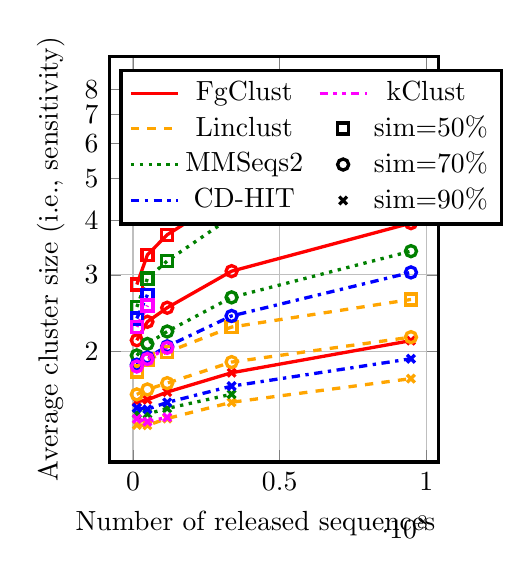
\begin{tikzpicture}
		\begin{axis}[very thick,grid=both,
		width=0.475\textwidth,height=0.555\textwidth,
		mark options={solid},
		%ymin=1,
		ymax=9.5, %7,%xmax=1.1e8,
		ymode=log,
		ytick={1,2,3,4,5,6,7,8},log ticks with fixed point,
		xlabel=Number of released sequences ~~~~,
		ylabel={Average cluster size (i.e., sensitivity)},
		legend columns=4,
		transpose legend,
		legend entries={FgClust~~,
			Linclust~~,
			MMSeqs2~~,
			CD-HIT~~,
			kClust~~,
			sim=50\%,sim=70\%,sim=90\%},
		legend pos=north west]
		\addlegendimage{,color=Red}
		\addlegendimage{dashed,color=Orange}
		\addlegendimage{dotted,color=Green}
		\addlegendimage{dash dot,color=Blue}
		\addlegendimage{dash dot dot,color=Magenta}
		\addlegendimage{only marks,mark=square}
		\addlegendimage{only marks,mark=o}
		\addlegendimage{only marks,mark=x}
		
		\addplot[color=Red,mark=square] coordinates {
			(1306318        , 1306318       / 458303)
			(4910948        , 4910948       / 1473070)
			(11659891       , 11659891      / 3144453)
			(33613081       , 33613081      / 7306576)
			(94756963       , 94756963      / 15630526)
		}; %FgClust 50
		\addplot[color=Red,mark=o] coordinates {
			(1306318        , 1306318       / 615387)
			(4910948        , 4910948       / 2097994)
			(11659891       , 11659891      / 4625378)
			(33613081       , 33613081      / 10989844)
			(94756963       , 94756963      / 24032649)
		}; %FgClust 70
		\addplot[color=Red,mark=x] coordinates {
			(1306318        , 1306318       / 851325)
			(4910948        , 4910948       / 3168436)
			(11659891       , 11659891      / 7221652)
			(33613081       , 33613081      / 18798319)
			(94756963       , 94756963      / 44723337)
		}; %FgClust 90
		
		\addplot[dashed,color=Orange,mark=square] coordinates {
			( 1306318,       1306318/       725566    )
			( 4910948,       4910948/       2562086   )
			(11659891,      11659891/       5847706   )
			(33613081,      33613081/       14766033        )
			(94756963,      94756963/       35983786        )
		}; %Linclust 50
		\addplot[dashed,color=Orange,mark=o] coordinates {
			( 1306318,       1306318/       819293    )
			( 4910948,       4910948/       3000298   )
			(11659891,      11659891/       6889416   )
			(33613081,      33613081/       17768118        )
			(94756963,      94756963/       43908412        )
		}; %Linclust 70
		\addplot[dashed,color=Orange,mark=x] coordinates {
			( 1306318,       1306318/       962908    )
			( 4910948,       4910948/       3625681   )
			(11659891,      11659891/       8306445   )
			(33613081,      33613081/       21974288        )
			(94756963,      94756963/       54672623        )
		};
		
		\addplot[dotted,color=Green,mark=square] coordinates {
			( 1306318,       1306318/       516052    )
			( 4910948,       4910948/       1670691   )
			(11659891,      11659891/       3611539   )
			(33613081,      33613081/       8247496 )
			(94756963,      94756963/       17763784        )
		}; % mmseqs2 50
		\addplot[dotted,color=Green,mark=o] coordinates {
			( 1306318,       1306318/       666575    )
			( 4910948,       4910948/       2358569   )
			(11659891,      11659891/       5244463   )
			(33613081,      33613081/       12622515        )
			(94756963,      94756963/       27872093        )
		};
		\addplot[dotted,color=Green,mark=x] coordinates {
			( 1306318,       1306318/       906871    )
			( 4910948,       4910948/       3415601   )
			(11659891,      11659891/       7874593   )
			(33613081,      33613081/       21060831        )
			%(94756963,      94756963/       77117011       ) % timeout
		};
		
		\addplot[dash dot,color=Blue,mark=square] coordinates {
			( 1303982 , 1303982 / 547396 )
			( 4908596 , 4908596 / 1818516 )
		};
		\addplot[dash dot,color=Blue,mark=o] coordinates {
			( 1303982 , 1303982 / 698797 )
			( 4908596 , 4908596 / 2532809 )
			( 11656604 , 11656604 / 5671408 )
			( 33606888 , 33606888 / 13921644 )
			( 94744006 , 94744006 / 31180026 )
		};
		\addplot[dash dot,color=Blue,mark=x] coordinates {
			( 1303982 , 1303982 / 878273 )
			( 4908596 , 4908596 / 3329592 )
			( 11656604 , 11656604 / 7627716 )
			( 33606888 , 33606888 / 20175146 )
			( 94744006 , 94744006 / 49205865 )
			
		};
	
		\addplot[dash dot dot,color=Magenta,mark=square] coordinates {
			( 1303982 , 1303982 / 572347 )
			( 4908596 , 4908596 / 1924257 )
		};
		\addplot[dash dot dot,color=Magenta,mark=o] coordinates {
			( 1303982 , 1303982 / 705456 )
			( 4908596 , 4908596 / 2552951 )
			( 11656604 , 11656604 / 5713855 )
		};
		\addplot[dash dot dot,color=Magenta,mark=x] coordinates {
			( 1303982 , 1303982 / 930527 )
			( 4908596 , 4908596 / 3556609 )
			( 11656604 , 11656604 / 8250898 )
		};
		\end{axis}
		\end{tikzpicture}
		&
		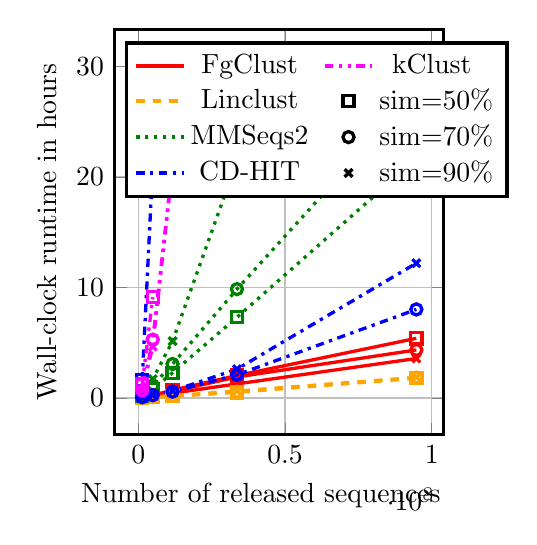
\begin{tikzpicture}
		\begin{axis}[very thick,grid=both,
		width=0.475\textwidth,height=0.555\textwidth,
		mark options={solid},
		%xmode=log,ymode=log,
		ymax=50/1.5,%xmax=1.1e8,
		xlabel=Number of released sequences ~~~~,
		ylabel=Wall-clock runtime in hours,
		legend columns=4,
		transpose legend, 
		legend entries={FgClust~~,
			Linclust~~,
			MMSeqs2~~,
			CD-HIT~~,
			kClust~~,
			sim=50\%,sim=70\%,sim=90\%},
		legend pos=north west
		]
		\addlegendimage{,color=Red}
		\addlegendimage{dashed,color=Orange}
		\addlegendimage{dotted,color=Green}
		\addlegendimage{dash dot,color=Blue}
		\addlegendimage{dash dot dot,color=Magenta}
		\addlegendimage{only marks,mark=square}
		\addlegendimage{only marks,mark=o}
		\addlegendimage{only marks,mark=x}
		
		\addplot[color=Red,mark=square] coordinates {
			( 1306318,      216.03 / 3600)
			( 4910948,      923.48 / 3600)
			(11659891,      2554.06 / 3600)
			(33613081,      7305.12 / 3600)
			(94756963,      19434.67 / 3600)
		};
		\addplot[color=Red,mark=o] coordinates {
			( 1306318,      164.24 / 3600)
			( 4910948,      712.02 / 3600)
			(11659891,      2151.47 / 3600)
			(33613081,      6858.06 / 3600)
			(94756963,      15651.55 / 3600)
		};
		\addplot[color=Red,mark=x] coordinates {
			( 1306318,      105.10 / 3600)
			( 4910948,      446.33 / 3600)
			(11659891,      1578.28 / 3600)
			(33613081,      4595.46 / 3600)
			(94756963,      12873.48 / 3600)
		};
	
		\addplot[dashed,color=Orange,mark=square] coordinates {
			( 1306318,      63.24 / 3600)
			( 4910948,      259.20 / 3600)
			(11659891,      600.11 / 3600)
			(33613081,      1859.28 / 3600)
			(94756963,      6444.66 / 3600)
		}; %linclust 50
		\addplot[dashed,color=Orange,mark=o] coordinates {
			( 1306318,      66.58 / 3600)
			( 4910948,      278.11 / 3600)
			(11659891,      652.31 / 3600)
			(33613081,      2013.65 / 3600)
			(94756963,      6639.85 / 3600)
		};
		\addplot[dashed,color=Orange,mark=x] coordinates {
			( 1306318,      73.96 / 3600)
			( 4910948,      334.20 / 3600)
			(11659891,      744.64 / 3600)
			(33613081,      2270.75 / 3600)
			(94756963,      6698.25 / 3600)
		};
		
		\addplot[dotted,color=Green,mark=square] coordinates {
			( 1306318,      603.10 / 3600)
			( 4910948,      2898.67 / 3600)
			(11659891,      8230.45 / 3600)
			(33613081,      26272.73 / 3600)
			(94756963,      77837.47 / 3600)
		};
		\addplot[dotted,color=Green,mark=o] coordinates {
			( 1306318,      737.74 / 3600)
			( 4910948,      4098.65 / 3600)
			(11659891,      11068.39 / 3600)
			(33613081,      35445.09 / 3600)
			(94756963,      99781.83 / 3600)
		};
		\addplot[dotted,color=Green,mark=x] coordinates {
			( 1306318,      905.05 / 3600)
			( 4910948,      6154.68 / 3600)
			(11659891,      18524.44 / 3600)
			(33613081,      77145.61 / 3600)
			%(94756963,timeout)
		};
		
		\addplot[dash dot,color=Blue,mark=square] coordinates {
			( 1306318,      5766.21 / 3600)
			( 4910948,      75911.85 / 3600)
			%(11659891,timeout)
			%(33613081,timeout)
			%(94756963,timeout)
		};
		\addplot[dash dot,color=Blue,mark=o] coordinates {
			( 1306318,      264.31 / 3600)
			( 4910948,      929.93 / 3600)
			(11659891,      2062.60 / 3600)
			(33613081,      7563.33 / 3600)
			(94756963,      28834.18 / 3600)
		};
		\addplot[dash dot,color=Blue,mark=x] coordinates {
			( 1306318,      311.15 / 3600)
			( 4910948,      955.40 / 3600)
			(11659891,      2315.58 / 3600)
			(33613081,      9395.35 / 3600)
			(94756963,      43880.61 / 3600)
		};
	
		\addplot[dash dot dot,color=Magenta,mark=square] coordinates {
			( 1303982 , 4378.45 / 3600 )
			( 4908596 , 32820.26 / 3600 )
		};
		\addplot[dash dot dot,color=Magenta,mark=o] coordinates {
			( 1303982 , 2447.86 / 3600 )
			( 4908596 , 19014.50 / 3600 )
			( 11656604 , 75912.68 / 3600 )
		};
		\addplot[dash dot dot,color=Magenta,mark=x] coordinates {
			( 1303982 , 2597.88 / 3600 )
			( 4908596 , 16724.53 / 3600 )
			( 11656604 , 75284.21 / 3600 )
		};
		\end{axis}
		\end{tikzpicture}
	\end{tabular}
	\caption{
		%This figure shows the impact of database growth on sensitivity and runtime.
		UniProt released
		\SI{1306318}{},
		\SI{4910948}{}, 
		\SI{11659891}{}, 
		\SI{33613081}{}, and 
		\SI{94756963}{} 
		sequences into 
		UniRef100-2.0,
		UniRef100-12.0,
		UniRef100-2011-01, 
		UniRef100-2014-01, and
		UniRef100-2017-01
		in 
		July 2004,
		July 2017,
		January 2011,
		January 2014, and
		January 2017,
		respectively \citep{suzek2007uniref}.
%		These five releases are referred to as UniRef100-2.0,
%		UniRef100-12.0,
%		UniRef100-2011-01, 
%		UniRef100-2014-01, and
%		UniRef100-2017-01, respectively \citep{suzek2007uniref}.
		We ran each program on each release of the UniRef100 database with each similarity cutoff to generate each set of clusters.
		Cluster quality is not evaluated due to the lack of ground truth. 
		Each program times out after running for \SI{50}{} hours.
		\label{fig:uniref}
	}
\end{figure}

\subsection{Evaluation on protein structures in PDB}

\begin{table}[t]%[!htbp]
	\centering
	\caption{
		The sequences of \SI{49686} monomeric proteins in PDB deposited exclusively before January 2\textsuperscript{nd} 2017 are given as input to each program \citep{berman2006protein}. 
		Each program is run with each similarity cutoff to generate each set of clusters.
		The template-modeling (TM) score between each representative cluster centroid and each sequence covered by the centroid is tabulated. A centroid trivially covers itself with a TM score of 1.
		%For each set of clusters, the number of sequences characterized by intra-cluster template-modeling (TM) scores inclusively below each threshold is tabulated.
		%The intra-cluster TM score of a cluster is the lowest TM score between the representative sequence in the cluster as template and each represented sequence in the cluster.
		%A cluster with an intra-cluster TM-score of at most 0.5 contains at least one outlier in terms of three-dimensional structure and thus is of bad quality 
		If the TM score is at most 0.5, then the centroid and covered sequence are usually significantly different in protein structure
		\cite{xu2010significant}.
		%FgClust generates the least number of bad-quality clusters.
		The wall-clock runtime of each program is too short to measure scalability.
	}
	\begin{tabular}{l c c c c c c c c c}
		\toprule
		Program & similarity  & number of & 
		\multicolumn{7}{c}{TM scores of centroids modeling covered sequences} \\
		& cutoff      & clusters  &
		~\(\le\) 0.3~ & ~\(\le\) 0.4~ & ~\(\le\) 0.5~
		& ~\(\le\) 0.6~ & ~\(\le\) 0.7~ & ~\(\le\) 0.8~ & ~\(\le\) 0.9~ \\
		\midrule
		
		FgClust   & 50\% & 14784 &  88 & 248 & {\bfseries 547} & 1149 & 2150 & 3855 & 8227 \\
		Linclust  & 50\% & 17381 & 166 & 390 & 708 & 1160 & 1854 & 3010 & 5831 \\
		MMSeqs2   & 50\% & 15160 & 226 & 515 & 938 & 1790 & 2862 & 4445 & 8651 \\
		CD-HIT    & 50\% & 15658 & 266 & 574 & 981 & 1697 & 2628 & 3961 & 7305 \\
		kClust    & 50\% & 16108 & 181 & 423 & 809 & 1404 & 2179 & 3505 & 6884 \\ 
		\noalign{\vskip 2mm} 
		FgClust   & 70\% & 17538 &  47 & 141 & {\bfseries 340} & 676  & 1285 & 2311 & 4387 \\
		Linclust  & 70\% & 18207 & 174 & 402 & 674 & 1083 & 1702 & 2709 & 4912 \\
		MMSeqs2   & 70\% & 17158 & 236 & 506 & 826 & 1355 & 2107 & 3209 & 5600 \\
		CD-HIT    & 70\% & 17610 & 242 & 464 & 751 & 1265 & 1956 & 2998 & 5308 \\
		kClust    & 70\% & 17682 & 187 & 405 & 695 & 1188 & 1811 & 2837 & 5244 \\
		\noalign{\vskip 2mm} 
		FgClust   & 90\% & 19993 &  17 & 66  & {\bfseries 169} & 346  & 736  & 1359 & 2975 \\
		Linclust  & 90\% & 19552 & 125 & 284 & 507 & 872  & 1378 & 2149 & 3834 \\
		MMSeqs2   & 90\% & 18783 & 219 & 426 & 734 & 1143 & 1810 & 2717 & 4669 \\
		CD-HIT    & 90\% & 19124 & 189 & 364 & 586 & 940  & 1485 & 2300 & 4041 \\
		kClust    & 90\% & 19707 & 141 & 315 & 513 & 848  & 1306 & 2128 & 3800 \\
		\bottomrule
	\end{tabular}
	\label{table:pdb}
\end{table}

We evaluated the sensitivity and specificity of FgClust by using three-dimensional alignments of experimentally determined protein structures.
We downloaded all monomeric proteins with experimentally determined structures deposited into PDB exclusively before January 2\textsuperscript{nd} 2017 \citep{berman2006protein}.
The sequence of each protein is extracted.
If an extracted sequence has at least 11 non-ambiguous amino acids and at least 90\% amino acids of the extracted sequence are non-ambiguous, then the extracted sequence is kept.
From these kept sequences, each sequence-clustering algorithm was used to generate a set of clusters.
Within each cluster, the template-modeling (TM) score between the representative sequence and each represented sequence is computed by TM-Align \citep{zhang2005tm}.
%The distribution of such TM scores is shown in \cref{table:pdb}.
A lower TM score means a lower specificity achieved by a clustering algorithm.
%The lower such TM scores are, the less specific the clustering algorithm is.
FgClust generates the fewest number of sequences with low TM scores (i.e., at most 0.5) to their centroids (\cref{table:pdb}).
Usually, two proteins are in the same fold if and only if these two proteins share a TM-score of more than 0.5 \citep{xu2010significant}, where a protein fold is defined by the arrangement of the secondary structure elements relative to each other in space.
%\Cref{table:pdb} shows 
%We found that other algorithms produce about 50\% more clusters with intra-cluster TM scores of at most 0.5 than FgClust.
%We found that FgClust generated clusters such that the least number of sequences.
As a result, FgClust is significantly more specific than other algorithms in terms of experimentally determined protein structures.
Furthermore, FgClust at 50\% similarity cutoff generates the fewest clusters with the highest average cluster size.
Therefore, FgClust is significantly more specific and sensitive than other algorithms in terms of protein structural similarity.
%Thus, FgClust can improve the protein-structure prediction based on homology-modeling, the structural classification of proteins, etc.
The better specificity and sensitivity of FgClust on PDB structures are attributed to the use of Murphy10 to reduce amino-acid alphabet and 25 residues to normalize edit-similarity, respectively (data not shown).

\subsection{Evaluation on protein families in Pfam}

\begin{figure}%[!htbp]
	\centering
	\begin{tabular}{c c}
		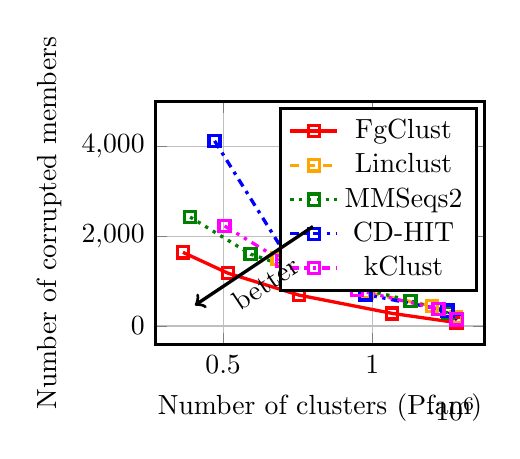
\begin{tikzpicture}
		\begin{axis}[very thick,grid=both,
		mark options={solid},
		width=0.475\textwidth,
		height=0.385\textwidth,
		ymax=5000,
		xlabel=Number of clusters (Pfam),
		ylabel=Number of corrupted members]
		\addplot[color=Red,mark=square] coordinates {
			(365172, 1642)
			(516422, 1177)
			(755086, 688)
			(1066591, 282)
			(1282334, 77)
		};
		\addlegendentry{FgClust}
		\addplot[dashed,color=Orange,mark=square] coordinates {
			(682422, 1501)
			(806160, 1111)
			(982978, 749)
			(1199664, 445)
			(1281061, 193)
		};
		\addlegendentry{Linclust}
		\addplot[dotted,color=Green,mark=square] coordinates {
			(389286, 2429)
			(592144, 1602)
			(843097, 1037)
			(1128443, 561)
			(1253416, 294)
		};
		\addlegendentry{MMSeqs2}
		\addplot[dash dot,color=Blue,mark=square] coordinates {
			(471396, 4126)
			(713570, 1549)
			(976870, 705)
			(1252062, 342)
			(1284604, 139)
		};
		\addlegendentry{CD-HIT}
		\addplot[dash dot dot,color=Magenta,mark=square] coordinates {
			(504834,2230)
			(697636,1452)
			(947935,804)
			(1221908,379)
			(1283087,149)
		};
		\addlegendentry{kClust}
		\end{axis}
		\draw[->,very thick](2,1.5)--(0.5,0.5)node
		[midway,below,sloped]{better};
		\end{tikzpicture}
		&
		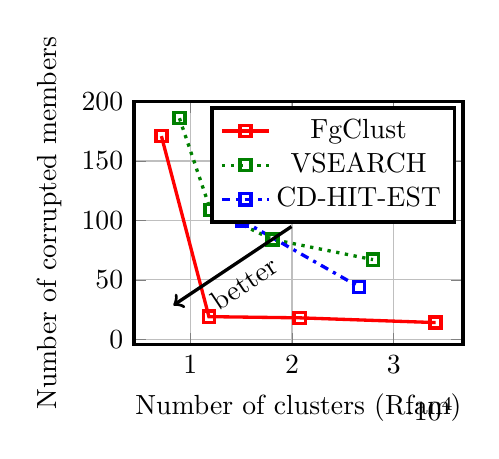
\begin{tikzpicture}
		\begin{axis}[very thick,grid=both,
		mark options={solid},
		width=0.475\textwidth,
		height=0.385\textwidth,
		ymax=200,%ymode=log,
		xlabel=Number of clusters (Rfam),
		ylabel=Number of corrupted members]
		\addplot[color=Red,mark=square] coordinates {
			%(4963, 3782)
			(7156, 171)
			(11828, 19)
			(20754, 18)
			(34117, 14)
		};
		\addlegendentry{FgClust}
		\addplot[dotted,color=Green,mark=square] coordinates {
			%(7509, 1958)
			(8929, 186)
			(11978, 109)
			(18085, 84)
			(27963, 67)
		};
		\addlegendentry{VSEARCH}
		\addplot[dash dot,color=Blue,mark=square] coordinates {
			(15074, 100)
			(26608, 44)
		};
		\addlegendentry{CD-HIT-EST}
		\end{axis}
		\draw[->,very thick](2,1.5)--(0.5,0.5)node
		[midway,below,sloped]{better};
		\end{tikzpicture}
	\end{tabular}
	\caption{Results of clustering Pfam-A-seed release 31.0 \citep{finn2016pfam} (left) and Rfam-seed release 12.3 \citep{nawrocki2014rfam} (right).
		On each plotted curve, the five marks from left to right correspond to the five sequence-similarity cutoffs of 50\% (only for Pfam), 60\%, 70\%, 80\%, and 90\%, respectively.
		CD-HIT-EST does not run with any sequence-similarity cutoff of less than 80\%.
		%A cluster is corrupted if and only if at least one member in the cluster is corrupted.
		A cluster member is corrupted if and only if the member belongs to a Pfam or Rfam family that the representative of the cluster does not belong to.
		The wall-clock runtime of each program is too short to measure scalability.
		\label{fig:pfam}
		\label{fig:rfam}
	}
\end{figure}

Pfam offers a benchmark for the classification of functional protein domains \citep{finn2016pfam}.
For this evaluation, we applied each clustering algorithm on
%Thus, we evaluated the sensitivity and specificity of clustering algorithms using Pfam.
%We downloaded 
the manually checked seed A dataset from Pfam release 31.0 \citep{finn2016pfam}.
%We ran each clustering algorithm on this dataset.
We assessed the quality of the clusters in terms of 
%the number of corrupted clusters and 
the number of corrupted sequences contained by a cluster.
%We consider a cluster to be corrupted if it contains at least two sequences that belong to two different Pfam families.
%Also, we
We regarded a sequence, or a member of a cluster, to be corrupted if it belongs to a Pfam family that the representative of the cluster does not belong to.
%A corrupted cluster member belongs to a Pfam family that the representative of this cluster does not belong to.
A more sensitive clustering algorithm generates fewer clusters, whereas a more specific clustering algorithm generates fewer corrupted cluster members.
As previously mentioned, 
the number of corrupted clusters (a corrupted cluster contains sequences belonging to different families) is not normalized against the input and is therefore not meaningful for measuring specificity.
However, the number of corrupted clusters can reveal the characteristics of different clustering algorithms and is therefore still shown in \cref{fig:pfam-appendix}.
We found that FgClust generates much fewer clusters given the same number of corrupted cluster members and much fewer corrupted cluster members given the same number of clusters (\cref{fig:pfam}).
The result shows that FgClust is significantly more sensitive at the same specificity and significantly more specific at the same sensitivity.
Therefore, FgClust achieves the best sensitivity-specificity trade-off.
%FgClust can improve protein-function prediction based on homology modeling, functional classification of proteins, the construction of Hidden Markov Models (HMMs) for protein families, etc.
The improved sensitivity of FgClust on Pfam-A-seed is probably due to the use of the Murphy10 reduced alphabet (data not shown).
The specificity of FgClust on Pfam-A-seed is mostly improved by the use of 25 residues to normalized edit-similarity (data not shown). 

At low sequence-similarity cutoffs (e.g., 50\%),
CD-HIT has the worst sensitivity-specificity trade-off, presumably because inferring biological similarity from a low sequence identity is highly error-prone.
FgClust normalizes edit-similarity with respect to sequence length.
Linclust, MMSeqs2, and kClust use e-value in addition to sequence identity.
As a result, FgClust, Linclust, MMSeqs2, and kClust do not suffer from a drop in sensitivity-specificity trade-off at a low sequence similarity.
Linclust, MMSeqs2, and kClust use iterative, profile-based clustering strategy and can thus merge similar clusters into one single cluster.
A false-positive merging step corrupts only one cluster, but it can corrupt multiple cluster members.
Thus, Linclust, MMSeqs2, and kClust generate high numbers of corrupted cluster members compared with the numbers of corrupted clusters (\cref{fig:pfam,fig:pfam-appendix}).

\subsection{Evaluation on RNA families in Rfam}

Rfam provides a gold-standard benchmark for the classification of non-coding RNA sequences \citep{nawrocki2014rfam}.
In this study, we utilized the manually checked seed dataset from Rfam release 12.3 \citep{nawrocki2014rfam}.
%Thus, we evaluated the sensitivity and specificity of clustering algorithms using Rfam. 
%We downloaded the manually checked seed dataset from Rfam release 12.3 \citep{nawrocki2014rfam}.
%We ran FgClust commit 93c3a6d9, VSEARCH v2.3.4\_linux\_x86\_64 \citep{rognes2016vsearch}, and CD-HIT-EST version 4.6 \citep{fu2012cd} on this dataset.
Evaluation metrics for Pfam and Rfam are similar.
%\Cref{fig:rfam} shows 
In our experiments, we found that FgClust generates much fewer clusters given the same number of corrupted cluster members and much fewer corrupted cluster members given the same number of clusters (\cref{fig:rfam}).
%Thus, FgClust is significantly more sensitive at the same specificity and significantly more specific at the same sensitivity.
This result indicates that FgClust achieves the best overall sensitivity-specificity trade-off.
%FgClust can improve RNA-function prediction based on homology modeling, functional classification of RNAs, the construction of HMMs for RNA families etc.
% improvement
%Additionally, the 
The sensitivity and specificity of FgClust on Rfam-seed is mostly improved by the use of edit-similarity instead of sequence identity as the cutoff (data not shown).
The specificity of FgClust on Rfam-seed is also improved by the use of 25 residues to normalized edit-similarity (data not shown).

\section{Conclusion}

We developed FgClust, a novel algorithm for clustering biological sequences.
FgClust is more sensitive, more specific, and faster than other state-of-the-art clustering algorithms, except that Linclust is two times faster but also generates up to more than 130\% more clusters than FgClust.
We observed that greedy incremental update may not select the optimal centroid during each incremental update.
Accordingly, FgClust detects a sufficient number of sequence pairs such that, in each pair, the first can represent the second.
Then, FgClust uses greedy set cover to cluster all sequences based on such pairings.
We observed that there are too many short words in a typical biological sequence.
Accordingly, FgClust uses min-hash values instead of short words as filter.
We observed that sequence identity is not sufficiently correlated with biological similarity and requires the time-consuming computation of alignment.
Accordingly, FgClust uses edit-similarity instead of sequence identity.
%Edit-similarity is defined as one minus the following: 
%	number of single-character edits to change a member sequence into a substring of the centroid sequence, divided by the length of the member sequence.

FgClust generates clusters of the highest quality. 
Consequently, FgClust reduces manual-curation efforts and errors in the downstream analysis of clusters.
For example, sequences in the same cluster can be assumed to be homologous to each other for homology modeling.
Errors in homology modeling are reduced by the use of FgClust.
This reduction in errors results in less manual examination of the errors and improves the prediction of structures and functions \citep{nayeem2006comparative}.
Moreover, FgClust is fast and scalable.
FgClust will be able to handle the large volume of sequences released by UniProt and metagenomic studies.

In the future, we will construct a Hidden Markov Model (HMM) for each cluster generated by FgClust and evaluate the quality of such HMMs.
Moreover, we will apply the techniques used in FgClust to other problems, such as metagenomics-sequence classification and chimera detection.%, and detection of conserved protein domains.

\bibliographystyle{plainnat}
%\bibliographystyle{unsrtnat}
\bibliography{clust}

\clearpage{}

\appendix

\section{Appendix}
\subsection{Canonical specificity is not normalized against input}
\label{sec:appendix:canonical-specificity}
Canonical clustering sensitivity is the average number of sequences in each cluster.
Canonical clustering specificity is either the percentage of clusters that are not corrupted \citep{hauser2013kclust} or the average consistency of each cluster \citep{hauser2016mmseqs,steinegger2017mmseqs2,steinegger2017linclust}.
By definition, all singletons (i.e., clusters that contain only one sequence per cluster) are not corrupted and are characterized by the highest consistency.
However, if a large number of input sequences are clustered into one large cluster and a large number of singletons, then the resulting clusters achieve both high canonical sensitivity and high canonical specificity.
For example, one million sequences can be partitioned into one thousand clusters such that one cluster contains \SI{999001} sequences and the other \SI{999} clusters contain one sequence each.
In this case, 
the canonical sensitivity is high because only one thousand clusters are generated out of one million sequences, 
and the canonical specificity is high because only the cluster containing \SI{999001} sequences is corrupted and/or not characterized by the highest consistency.
As a result, canonical specificity is not normalized against the input and is therefore not meaningful for measuring specificity.

\clearpage{}

\begin{table}[t]%[!htbp]
	\centering
	\caption{
		Extension of \cref{table:pdb} to include canonical specificity.
		In this case, canonical specificity is measured by intra-cluster template-modeling (TM) score.
		%The sequences of \SI{49686} monomeric proteins in PDB deposited exclusively before January 2\textsuperscript{nd} 2017 are given as input to each program \citep{berman2006protein}. 
		%Each program is run with each similarity cutoff to generate each set of clusters.
		The intra-cluster TM score of a cluster is the lowest TM score between the representative sequence in the cluster as template and each represented sequence in the cluster.
		For each set of clusters, the number of sequences characterized by intra-cluster TM scores inclusively below each threshold is tabulated.
		%A cluster with an intra-cluster TM-score of at most 0.5 contains at least one outlier in terms of three-dimensional structure and thus is of bad quality 
		%If the TM score is at most 0.5, then the centroid and covered sequence are significantly different in protein structure
		%\cite{xu2010significant}.
		%FgClust generates the least number of bad-quality clusters.
		%The wall-clock runtime of each program is too short to measure scalability.
	}
	\begin{tabular}{l c c c c c c c c c c}
		\toprule
		Program & similarity & 
		\multicolumn{8}{c}{intra-cluster TM scores} \\
		& cutoff      & ~\(\le\)0.2~ &
		~\(\le\)0.3~ & ~\(\le\)0.4~ & ~\(\le\)0.5~ 
		& ~\(\le\)0.6~ & ~\(\le\)0.7~ & ~\(\le\)0.8~ & ~\(\le\)0.9~ & ~\(\le\)1~ \\
		\midrule
		
		FgClust & 50 & 4 & 60 & 143 & 283 & 565 & 1020 & 1639 & 2606 & 14784 \\
		Linclust & 50 & 28 & 108 & 232 & 380 & 617 & 975 & 1490 & 2298 & 17381 \\
		MMSeqs2 & 50 & 32 & 132 & 263 & 424 & 701 & 1113 & 1654 & 2499 & 15160 \\
		CD-HIT & 50 & 44 & 139 & 281 & 438 & 695 & 1114 & 1634 & 2440 & 15658 \\
		kClust & 50 & 29 & 114 & 250 & 397 & 628 & 1017 & 1530 & 2351 & 16108 \\
		\noalign{\vskip 2mm} 
		FgClust & 70 & 3 & 29 & 83 & 181 & 380 & 714 & 1208 & 1991 & 17538 \\
		Linclust & 70 & 28 & 110 & 225 & 360 & 577 & 907 & 1382 & 2123 & 18207 \\
		MMSeqs2 & 70 & 32 & 127 & 251 & 391 & 629 & 995 & 1475 & 2236 & 17158 \\
		CD-HIT & 70 & 41 & 129 & 247 & 380 & 592 & 923 & 1398 & 2121 & 17610 \\
		kClust & 70 & 29 & 113 & 228 & 366 & 560 & 881 & 1335 & 2063 & 17682 \\
		\noalign{\vskip 2mm} 
		FgClust & 90 & 2 & 9 & 31 & 90 & 197 & 401 & 739 & 1420 & 19993 \\
		Linclust & 90 & 20 & 85 & 177 & 302 & 479 & 763 & 1175 & 1889 & 19552 \\
		MMSeqs2 & 90 & 35 & 111 & 217 & 358 & 549 & 826 & 1252 & 1962 & 18783 \\
		CD-HIT & 90 & 33 & 115 & 226 & 344 & 517 & 782 & 1171 & 1852 & 19124 \\
		kClust & 90 & 28 & 97 & 194 & 307 & 471 & 725 & 1083 & 1732 & 19707 \\
		
		\bottomrule
	\end{tabular}
	\label{table:pdb-appendix}
\end{table}



\begin{figure}%[!htbp]
	\centering
	\begin{tabular}{c c}
		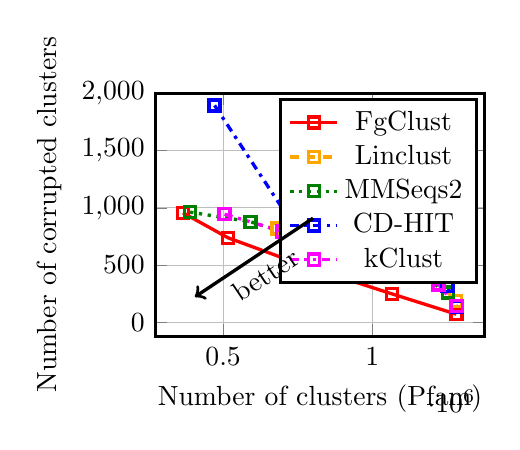
\begin{tikzpicture}
		\begin{axis}[very thick,grid=both,
		mark options={solid},
		width=0.475\textwidth,
		height=0.385\textwidth,
		ymax=2000,
		xlabel=Number of clusters (Pfam),
		ylabel=Number of corrupted clusters]
		\addplot[color=Red,mark=square] coordinates {
			(365172, 956)
			(516422, 738)
			(755086, 510)
			(1066591, 248)
			(1282334, 71)
		};
		\addlegendentry{FgClust}
		\addplot[dashed,color=Orange,mark=square] coordinates {	
			(682422, 819)
			(806160, 726)
			(982978, 572)
			(1199664, 401)
			(1281061, 188)
		};
		\addlegendentry{Linclust}
		\addplot[dotted,color=Green,mark=square] coordinates {
			(389286, 962)
			(592144, 878)
			(843097, 670)
			(1128443, 462)
			(1253416, 260)
		};
		\addlegendentry{MMSeqs2}
		\addplot[dash dot,color=Blue,mark=square] coordinates {
			(471396, 1894)
			(713570, 936)
			(976870, 558)
			(1252062, 317)
			(1284604, 135)
		};
		\addlegendentry{CD-HIT}
		\addplot[dash dot dot,color=Magenta,mark=square] coordinates {
			(504834,944)
			(697636,794)
			(947935,578)
			(1221908,331)
			(1283087,141)
		};
		\addlegendentry{kClust}
		\end{axis}
		\draw[->,very thick](2,1.5)--(0.5,0.5)node
		[midway,below,sloped]{better};
		\end{tikzpicture}
		&
		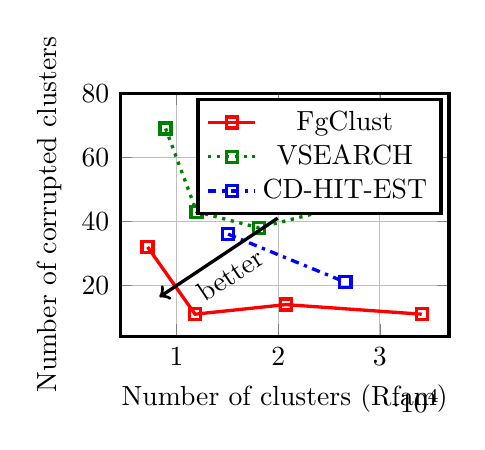
\begin{tikzpicture}
		\begin{axis}[very thick,grid=both,
		mark options={solid},
		width=0.475\textwidth,
		height=0.385\textwidth,
		ymax=80,%ymode=log,
		xlabel=Number of clusters (Rfam),
		ylabel=Number of corrupted clusters]
		\addplot[color=Red,mark=square] coordinates {
			%(4963, 1458)
			(7156, 32)
			(11828, 11)
			(20754, 14)
			(34117, 11)
		};
		\addlegendentry{FgClust}
		\addplot[dotted,color=Green,mark=square] coordinates {
			%(7509, 126)
			(8929, 69)
			(11978, 43)
			(18085, 38)
			(27963, 46)
		};
		\addlegendentry{VSEARCH}
		\addplot[dash dot,color=Blue,mark=square] coordinates {
			(15074, 36)
			(26608, 21)
		};
		\addlegendentry{CD-HIT-EST}
		\end{axis}
		\draw[->,very thick](2,1.5)--(0.5,0.5)node
		[midway,below,sloped]{better};
		\end{tikzpicture}
	\end{tabular}
	\caption{
	Extension of \cref{fig:pfam} to include canonical specificity.
	%Results of clustering Pfam-A-seed release 31.0 \citep{finn2016pfam} (left) and Rfam-seed release 12.3 \citep{nawrocki2014rfam} (right).
	%On each plotted curve, the five marks from left to right correspond to the five sequence-similarity cutoffs of 50\% (only for Pfam), 60\%, 70\%, 80\%, and 90\%, respectively.
	In this case, canonical specificity is high if and only the number of corrupted clusters is low.
	A cluster is corrupted if and only if at least one member in the cluster belongs to a Pfam or Rfam family that the representative of the cluster does not belong to.
	%A cluster member is corrupted if and only if the member belongs to a Pfam or Rfam family that the representative of the cluster does not belong to.
	%The wall-clock runtime of each program is too short to measure scalability.
	\label{fig:pfam-appendix}
	}
\end{figure}












\iffalse

\begin{figure}%[!htbp]
	\centering
	\begin{tabular}{c c}
		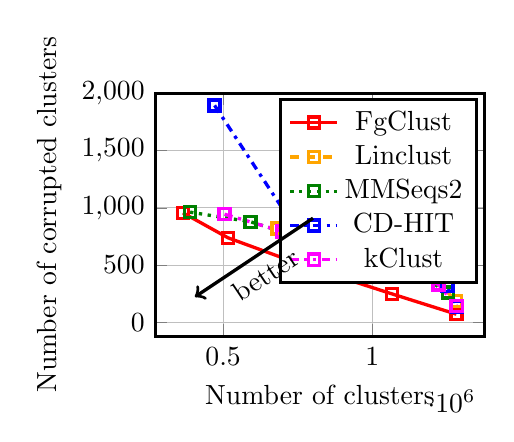
\begin{tikzpicture}
		\begin{axis}[very thick,grid=both,
		mark options={solid},
		width=0.475\textwidth,
		height=0.385\textwidth,
		ymax=2000,
		xlabel=Number of clusters,
		ylabel=Number of corrupted clusters]
		\addplot[color=Red,mark=square] coordinates {
			(365172, 956)
			(516422, 738)
			(755086, 510)
			(1066591, 248)
			(1282334, 71)
		};
		\addlegendentry{FgClust}
		\addplot[dashed,color=Orange,mark=square] coordinates {	
			(682422, 819)
			(806160, 726)
			(982978, 572)
			(1199664, 401)
			(1281061, 188)
		};
		\addlegendentry{Linclust}
		\addplot[dotted,color=Green,mark=square] coordinates {
			(389286, 962)
			(592144, 878)
			(843097, 670)
			(1128443, 462)
			(1253416, 260)
		};
		\addlegendentry{MMSeqs2}
		\addplot[dash dot,color=Blue,mark=square] coordinates {
			(471396, 1894)
			(713570, 936)
			(976870, 558)
			(1252062, 317)
			(1284604, 135)
		};
		\addlegendentry{CD-HIT}
		\addplot[dash dot dot,color=Magenta,mark=square] coordinates {
			(504834,944)
			(697636,794)
			(947935,578)
			(1221908,331)
			(1283087,141)
		};
		\addlegendentry{kClust}
		\end{axis}
		\draw[->,very thick](2,1.5)--(0.5,0.5)node
		[midway,below,sloped]{better};
		\end{tikzpicture}
		&
		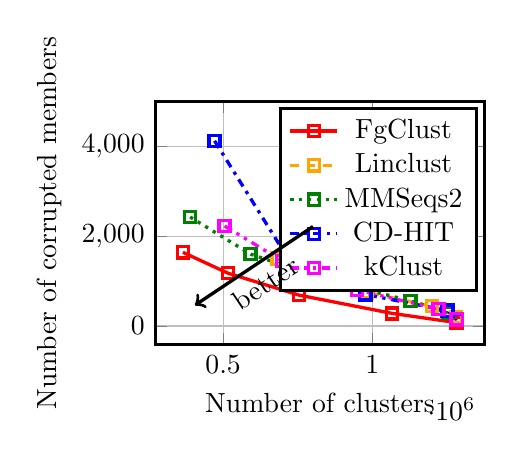
\begin{tikzpicture}
		\begin{axis}[very thick,grid=both,
		mark options={solid},
		width=0.475\textwidth,
		height=0.385\textwidth,
		ymax=5000,
		xlabel=Number of clusters,
		ylabel=Number of corrupted members]
		\addplot[color=Red,mark=square] coordinates {
			(365172, 1642)
			(516422, 1177)
			(755086, 688)
			(1066591, 282)
			(1282334, 77)
		};
		\addlegendentry{FgClust}
		\addplot[dashed,color=Orange,mark=square] coordinates {
			(682422, 1501)
			(806160, 1111)
			(982978, 749)
			(1199664, 445)
			(1281061, 193)
		};
		\addlegendentry{Linclust}
		\addplot[dotted,color=Green,mark=square] coordinates {
			(389286, 2429)
			(592144, 1602)
			(843097, 1037)
			(1128443, 561)
			(1253416, 294)
		};
		\addlegendentry{MMSeqs2}
		\addplot[dash dot,color=Blue,mark=square] coordinates {
			(471396, 4126)
			(713570, 1549)
			(976870, 705)
			(1252062, 342)
			(1284604, 139)
		};
		\addlegendentry{CD-HIT}
		\addplot[dash dot dot,color=Magenta,mark=square] coordinates {
			(504834,2230)
			(697636,1452)
			(947935,804)
			(1221908,379)
			(1283087,149)
		};
		\addlegendentry{kClust}
		\end{axis}
		\draw[->,very thick](2,1.5)--(0.5,0.5)node
		[midway,below,sloped]{better};
		\end{tikzpicture}
	\end{tabular}
	\caption{Results of clustering Pfam-A-seed release 31.0 \citep{finn2016pfam} (left) and Rfam-seed release 12.3 \citep{nawrocki2014rfam} (right).
		On each plotted curve, the five marks from left to right correspond to the five sequence-similarity cutoffs of 50\% (only for Pfam), 60\%, 70\%, 80\%, and 90\%, respectively.
		%A cluster is corrupted if and only if at least one member in the cluster is corrupted.
		A cluster member is corrupted if and only if the member belongs to a Pfam or Rfam family that the representative of the cluster does not belong to.
		The wall-clock runtime of each program is too short to measure scalability.
		\label{fig:pfam-appendix}
	}
\end{figure}

\begin{figure}%[!htbp]
	\centering
	\begin{tabular}{c c}
		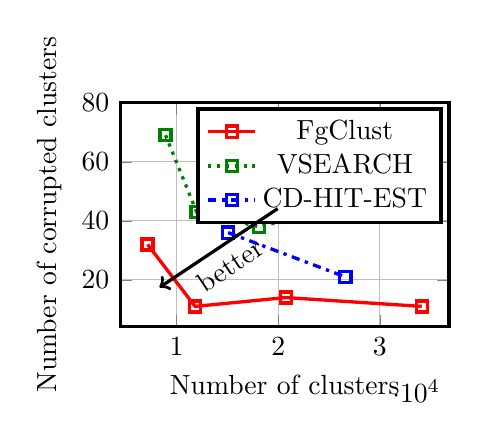
\begin{tikzpicture}
		\begin{axis}[very thick,grid=both,
		mark options={solid},
		width=0.475\textwidth,
		height=0.365\textwidth,
		ymax=80,%ymode=log,
		xlabel=Number of clusters,
		ylabel=Number of corrupted clusters]
		\addplot[color=Red,mark=square] coordinates {
			%(4963, 1458)
			(7156, 32)
			(11828, 11)
			(20754, 14)
			(34117, 11)
		};
		\addlegendentry{FgClust}
		\addplot[dotted,color=Green,mark=square] coordinates {
			%(7509, 126)
			(8929, 69)
			(11978, 43)
			(18085, 38)
			(27963, 46)
		};
		\addlegendentry{VSEARCH}
		\addplot[dash dot,color=Blue,mark=square] coordinates {
			(15074, 36)
			(26608, 21)
		};
		\addlegendentry{CD-HIT-EST}
		\end{axis}
		\draw[->,very thick](2,1.5)--(0.5,0.5)node
		[midway,below,sloped]{better};
		\end{tikzpicture}
		
		&
		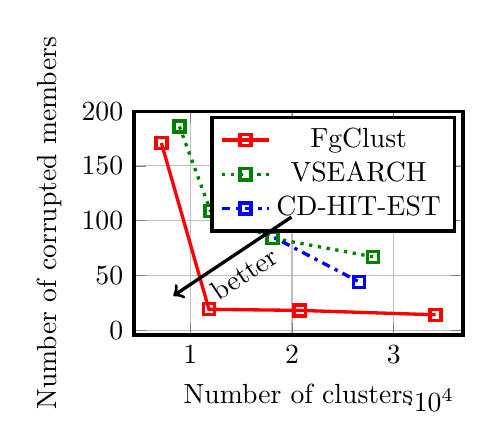
\begin{tikzpicture}
		\begin{axis}[very thick,grid=both,
		mark options={solid},
		width=0.475\textwidth,
		height=0.365\textwidth,
		ymax=200,%ymode=log,
		xlabel=Number of clusters,
		ylabel=Number of corrupted members]
		\addplot[color=Red,mark=square] coordinates {
			%(4963, 3782)
			(7156, 171)
			(11828, 19)
			(20754, 18)
			(34117, 14)
		};
		\addlegendentry{FgClust}
		\addplot[dotted,color=Green,mark=square] coordinates {
			%(7509, 1958)
			(8929, 186)
			(11978, 109)
			(18085, 84)
			(27963, 67)
		};
		\addlegendentry{VSEARCH}
		\addplot[dash dot,color=Blue,mark=square] coordinates {
			(15074, 100)
			(26608, 44)
		};
		\addlegendentry{CD-HIT-EST}
		\end{axis}
		\draw[->,very thick](2,1.5)--(0.5,0.5)node
		[midway,below,sloped]{better};
		\end{tikzpicture}
	\end{tabular}
	\caption{Results of clustering Rfam-seed release 12.3 \citep{nawrocki2014rfam}.
		On each plotted curve, the four marks from left to right correspond to the four sequence-similarity cutoffs of 60\%, 70\%, 80\%, and 90\%, respectively. CD-HIT-EST does not run with any sequence-similarity cutoff of less than 80\%.
		A cluster is corrupted if and only if at least one member in the cluster is corrupted.
		A cluster member is corrupted if and only if the member belongs to an Rfam family that the representative of the cluster does not belong to.
		The wall-clock runtime of each program is too short to measure scalability.
		\label{fig:rfam}
	}
\end{figure}

\subsection{Reduction of greediness in greedy incremental update}

Greedy incremental update may not be optimal.
For example, suppose we would like to cluster the following sequences at 65\% sequence identity:
ABXXEFGHIJ, 
ABXXEFXXI, and
BCDEFXXIJ.
In this case, 65\% sequence identity corresponds to 6 inclusive matches, or equivalently, exclusive edit distance of 4.
Then, greedy incremental update would pick ABXXEFGHIJ as the centroid of the first cluster, 
assign ABXXEFXXI to the first cluster because ABXXEFXXI is 3 edit distance away from ABXXEFGHIJ, 
and pick BCDEFXXIJ as the centroid of the second cluster because BCDEFXXIJ is 4 edit distance away from ABXXEFGHIJ.
However, if ABXXEFXXI is picked as the centroid of the first cluster, then both ABXXEFGHIJ and BCDEFXXIJ would be assigned to the first cluster. 

Instead of performing clustering while iterating through all sequences, we can perform clustering after computing the pairwise sequence identity of all sequences. 
In this case, sequence clustering is formulated as a dominating set problem, which is a special type of the set-cover problem. 
In this dominating set problem, an edge from a first vertex to a second vertex means that the first corresponding biological sequence can represent the second corresponding biological sequence. 

However, we observed that, for biological databases such as uniprot, the number of edges is orders of magnitude more numerous than the number of vertices. Thus, exhaustive generation of all edges requires substantial computational resources.
At the same time, such biological databases induce graphs characterized by rare cliques of large sizes, presumably because some biomolecules are over-represented due to their biological importance and/or abundance.
Thus, if an unvisited sequence is already represented by many other visited sequences that approximately form a clique, then this unvisited sequence is unlikely to form a new cluster that can contain members outside of this clique. 
Thus, in this case, we do not determine the sequences that this new sequence can represent, and thus do not generate any edge starting from the vertex corresponding to this new sequence. 
Thus, the resulting graph is incomplete but does not substantially affect the optimality of the resulting dominating set problem.

Then, we the greedy set-cover algorithm to solve the dominating set problem on the incomplete graph.
In addition of producing a solution that consists of a set of sequences, 
our greedy set-cover algorithm makes sure that each sequence is only represented by the best representative sequence.
For example, if sequence A can be represented by either representative sequences B or C but A is more similar to C,
then A will be clustered with C.
Our greedy set-cover algorithm uses linear memory and runtime and is highly optimized for memory usage.

\subsection{Throw-away of abundant and uninformative long words}

Some biological sequences contain uninformative region.
For example, a peptide sequence may consist of conserved regions and hypervariable regions.
The higher the sequence identity threshold is, the less informative the conserved region is.
Thus, two sufficiently dissimilar sequences can still share the same long word in the uninformative region.
If we use a naive long-word filter, then we will initiate a computationally more expensive comparison between these two sequences that share at least one uninformative long word.
An uninformative long word slows down the clustering process only if many sequences share this long word.
Thus, we rank all long words by percentile in increasing order of abundance.
For each long word that is longer than expected, we used hashed signatures, which are similar to short words in terms of function but are much less computationally intensive to work with, to estimate the sequence identity between some random pairs of sequences sharing this long word.
If the frequency that the estimated sequence identity meets the user-defined threshold is below a certain threshold,
then we throw-away the long word.
A throw-away long word does not initiate further computationally more expensive comparison between two sequences that share this long word.
Thus, computation time can be saved by removing uninformative long words without much sacrifice in sensitivity.
To reduce memory usage, we use the hash values of long words instead of the long words themselves, which is similar to the technique used in \citet{steinegger2017Linclust}.

\subsection{Reduction of short words into hashed signature}

A typical protein sequence consists of about 400 amino acids.
Thus, two protein sequences typically have two sets of 400 short words each.
However, if we uniformly, randomly, and independently (URI) subsample a small number of short words in each set of short words, then the subsampled short words can still work reasonably well. 
Nonetheless, we still need to maximize the collision rate between two sets of URI subsampled short words.
We used a technique similar to min-hash to achieve such URI subsampling while maximizing such collision rate.
In brief, each short word is hashed into a 16-bit unsigned integer.
The 31 smallest hash values form the signature of the sequence.
When we need to compare two sequences, we first compare their signatures.
If their signatures do not share a certain number of hash values in common, then we stop any further comparison between the two sequences. 
Otherwise, we proceed to compare the two sequences by using a computationally more expensive method.
Instead of comparing 400 short words, we only have to compare 31 hash values.

A typical nucleotide sequences is usually three times as long as a typical protein sequence.
Thus, the reduction of short words into signature is even more effective for nucleotide sequences.

One-to-many query-to-target sequence comparison is needed in sequence clustering. 
Similar to the technique used in \citet{li2006cd}, we sort, in descending order, the targets according to their number of shared hash values with the query before iterating through the targets. 
Similar to the technique used in \citet{edgar2010search}, we keep track of the number of failed attempts, or equivalently number of false-positive hits, when iterating through targets.
In addition, we keep track of the number of successful attempts, or equivalently number of true-positive hits, while iterating through targets.
Before iterating through the sorted targets, we initialize the number of remaining attempts to a positive integer.
If an attempt fails, we decrement the number of remaining attempts by one.
If an attempt succeeds, we increment the number of remaining attempts by a positive integer.
If the number of attempts becomes zero, then we stop iterating through the targets, because the not-yet-iterated remaining targets are not likely to be true positive hits.
The idea is that the ratio of success to failure should be above a certain threshold given a Bayesian prior of such ratio.

\subsection{Use of edit similarity instead of sequence identity}

Pairwise sequence identity is defined as the number of identical residues in a pairwise sequence alignment, divided by either the length of the alignment or the length of the shortest sequence. 
Unless explicitly stated otherwise, we assume that the sequence alignment used to generate sequence identity is the optimal alignment in terms of alignment score.

We developed a new measure of similarity between two sequences called edit-similarity.
The edit-similarity between a query and a target is defined as: the length of the target minus the number of edits required such that the target is a substring of the query, divided by the length of the target.
In terms of definition, edit-similarity is almost identical to the similarity in table 1 of \cite{vsovsic2017edlib}, 
except that edit-similarity uses target length as divisor whereas the similarity in \cite{vsovsic2017edlib} uses min(query-length, target-length) as the divisor. 
For example, the edit-similarity between \texttt{ACGGT} and \texttt{ATGG} is (4-1)/4, and the edit-similarity between \texttt{ATGG} and \texttt{ACGGT} is (5-2)/5.
The query is said to cover the target if the edit-similarity between the query and the target is higher than a predefined threshold.

Edit-distance requires much less computational time than pairwise alignment with substitution matrix, gap opening penalty, and gap extension penalty \cite{vsovsic2017edlib}. 
At first glance, it seems that we would lose some information by not computing pairwise alignment. 
However, it turns out that edit-similarity is biologically more relevant than sequence identity.
In the next two paragraphs, we will heuristically explain why edit-similarity is biologically more relevant.
In \ref{fig:specificity}, we will show that edit-similarity is more correlated with protein structural similarity than sequence identity.

Let \(s_1\) and \(s_2\) be two sequences such that \(s_1\) is longer than \(s_2\).
Let \(I(s_1, s_2)\) be the sequence identity between \(s_1\) and \(s_2\).
Let \(E(s_1, s_2)\) be the edit-similarity between \(s_1\) and \(s_2\).
If \(I(s_1, s_2) < E(s_1, s_2)\), then the alignment used to generate \(I(s_1, s_2)\) has fewer matches of identical residues, but more alignment score, than the alignment used to generate \(E(s_1, s_2)\).
Thus, the alignment used to generate \(I(s_1, s_2)\) must have in general more conserved amino-acid substitutions than the alignment used to generate \(E(s_1, s_2)\) in order to produce higher alignment score with less sequence identity.
However, the more conserved amino-acid substitutions from \(I(s_1, s_2)\) imply that \(I(s_1, s_2)\) probably underestimates the true biological similarity between \(s_1\) and \(s_2\) anyway, because more conserved amino-acid substitutions have bigger impact on protein structures and functions.
Thus, \(E(s_1, s_2)\) measures better the true biological similarity between \(s_1\) and \(s_2\) than \(I(s_1, s_2)\) even though the alignment used to compute \(I(s_1, s_2)\) can provide a white-box explanation for the relationship between \(s_1\) and \(s_2\).
For example, suppose \(s_1 = \texttt{AIAISSRRSSWWW}\) and \(s_2 = \texttt{AIAIWWW}\), 
and suppose we use BLOSUM62 matrix for computing \(I(s_1, s_2)\).
In BLOSUM62, the match reward for \texttt{W} is 11, and the match reward for both \texttt{A} and \texttt{I} is 4.
Thus, \(I(s_1, s_2) = 4/7\) because the           chunk \texttt{AIAI} is shared between \(s_1\) and \(s_2\).
but \(E(s_1, s_2) = 3/7\) because the conserved chunk \texttt{WWW}  is shared between \(s_1\) and \(s_2\).
However, since \texttt{W} is so conserved, \(3/7\) is an underestimates of the extend of biological relationship between \(s_1\) and \(s_2\).
Thus, \(4/7\) is closer to such extend of biological relationship.

Edit similarity is supposed to be uncorrelated with conservation of amino-acid residues, but sequence identity can be negatively correlated with conservation of amino-acid residues.
In addition, edit similarity considers deletion of \(s_1\) in \(s_2\), whereas sequence identity ignores deletion of \(s_1\) in \(s_2\).
For example, the edit similarity between \texttt{AAACGGG} and \texttt{AAAGGG} is (6-1)/6, but the corresponding sequence identity is 1. Thus, edit similarity is supposed to be more informative than sequence identity if part of the longer sequence is deleted in the shorter sequence.

\fi

\end{document}
